\Subsection{Условные математические ожидания}

\begin{definition}
    $(\Omega, \mathcal{F}, P)$ - вероятностное пространство, $\xi : \Omega \to \mathbb{R}$ и $\mathbb{E} |\xi| < +\infty$. Пусть $\mathcal{A} \subset \mathcal{F}$ и $\mathcal{A}$ - $\sigma-$алгебра.

    $\mathbb{E} (\xi | \mathcal{A}) = \eta \, : \, \Omega \to \mathbb{R}$ - случайная величина, которая:

    \begin{enumerate}
        \item измерима относительно $\mathcal{A}$
        \item $\forall \, A \in \mathcal{A} \, : \, \mathbb{E} (\xi \mathds{1}_A) = \mathbb{E} (\eta \mathds{1}_A)$
    \end{enumerate}
\end{definition}

\begin{theorem}
    $\mathcal{A} \subset \mathcal{F}, \mathbb{E} |\xi| < +\infty$, тогда $\mathbb{E} (\xi | \mathcal{A})$ существует и единственно, с точностью до почти наверное
\end{theorem}

\begin{proof}
    \textbf{Существование}:

    $\xi = \xi_+ - \xi_-$. Пусть $A \in \mathcal{A}$, определим $\mu_{\pm} A = \int_A \xi_{\pm} \, dP$ - это конечные меры на $\mathcal{A}$, так как интеграл от измеримой неотрицательной функции.
    А ещё эти меры абсолютно непрерывны относительно $P \overset{\text{т. Радона-Никодима}}{\implies} \exists \, \eta_{\pm} > 0$ измеримые относительно $\mathcal{A}$, т.ч. $\mu_{\pm} A = \int_A \eta_{\pm} \, dP$
    
    $\eta = \eta_+ - \eta_-$, надо проверить, что $\forall \, A \in \mathcal{A} \, : \, \underbrace{\mathbb{E} (\xi \mathds{1}_A)}_{\mathbb{E}(\xi_+ \mathds{1}_A) - \mathbb{E}(\xi_- \mathds{1}_A)} = \mathbb{E} (\eta \mathds{1}_A)$

    А ещё $\mathbb{E}(\xi_+ \mathds{1}_A) = \mu_+ A = \int_A \xi_+ \, dP$ и для остальных точно также

    \textbf{Единственность}:

    Пусть $\eta_1$ и $\eta_2$ - условные матожидания. Тогда $\{ \eta_1 > \eta_2 \} \in \mathcal{A}$

    $\mathbb{E} (\eta_1 \mathds{1}_A) = \mathbb{E} (\xi \mathds{1}_A) = \mathbb{E} (\eta_2 \mathds{1}_A) \implies \underbrace{\mathbb{E} ((\eta_1 - \eta_2) \mathds{1}_A)}_{=\int_A (\eta_1 - \eta_2) \, dP} = 0 \implies P(A) = P(\eta_1 > \eta_2) = 0$. Аналогично $P(\eta_1 < \eta_2) = 0$
\end{proof}

\begin{properties}
    \begin{enumerate}
        \item $\mathbb{E} (c | \mathcal{A}) = c$
        \item $\mathbb{E} (\xi | \mathcal{A})$ линейно по $\xi$
        \item {$\xi \leqslant \eta$, то $\mathbb{E} (\xi | \mathcal{A}) \leqslant \mathbb{E} (\eta | \mathcal{A})$
            \begin{proof}
                Достаточно проверить, что если $\xi \geqslant 0$, то $\mathbb{E} (\xi | \mathcal{A}) \geqslant 0$
            \end{proof}
        }
        \item {
            $\mathbb{E} (\xi | \{ \emptyset, \Omega \}) = \mathbb{E} \xi$

            \begin{proof}
                Измеримы относительно такой $\sigma$-алгебры только константы. Надо проверить, что $\mathbb{E} (\mathbb{E} \xi \mathds{1}_A) = \mathbb{E} (\xi \mathds{1}_A)$ для $A = \emptyset$ и $A = \Omega$
            \end{proof}
        }
        \item {
            $\mathcal{F} \supset \mathcal{A}_1 \supset \mathcal{A}_2$ - $\sigma$-алгебры

            Тогда $\mathbb{E} (\mathbb{E} (\xi | \mathcal{A}_1) | \mathcal{A}_2) = \mathbb{E} (\xi | \mathcal{A}_2)$

            \begin{proof}
                $\eta = \mathbb{E} (\xi | \mathcal{A}_2)$ и $\zeta = \mathbb{E} (\xi | \mathcal{A}_1)$

                Надо доказать, что $\eta = \mathbb{E} (\zeta | \mathcal{A}_2)$. $\eta$ измерима относительно $\mathcal{A_2}$. Надо проверить, что 
                $\forall \, A \in \mathcal{A}_2 \, : \, \mathbb{E} (\eta \mathds{1}_A) = \mathbb{E} (\zeta \mathds{1}_A) = \mathbb{E} (\xi \mathds{1}_A)$, т.к. $A \in \mathcal{A}_1$ по определению $\zeta$. А ещё
                $\mathbb{E} (\xi \mathds{1}_A) = \mathbb{E} (\eta \mathds{1}_A)$
            \end{proof}
        }
        \item {
            $\mathbb{E} (\mathbb{E} (\xi | \mathcal{A})) = \mathbb{E} \xi$ - из $4$ и $5$
        }
        \item {
            Если $\xi$ измерима относительно $\mathcal{A}$, то $\mathbb{E} (\xi | \mathcal{A}) = \xi$
        }
    \end{enumerate}
\end{properties}

\begin{example}
    Пусть $\Omega = \bigsqcup A_k$  не более чем счётное объединение

    $\mathcal{A}$ - натянутая на $A_1, A_2, \ldots$ $\sigma-$алгебра

    $\mathbb{E} (\xi | \mathcal{A}) = ?$

    Если $\eta$ измерима относительно $\mathcal{A} \implies \eta = \sum c_k \mathds{1}_{A_k}$

    Нужно чтобы $\mathbb{E} (\xi \mathds{1}_{A_n}) = \mathbb{E} (\underbrace{\eta \mathds{1}_{A_n}}_{c_n \mathds{1}_{A_n}}) = c_n P(A_n)$

    То есть $c_n = \frac{\mathbb{E} (\xi \mathds{1}_{A_n})}{P(A_n)}$

    \begin{remark}
        Из свойства 6: $\mathbb{E} \xi = \mathbb{E} \eta = \sum \frac{\mathbb{E} (\xi \mathds{1}_{A_k})}{P(A_k)} \cdot P(A_k)$
    \end{remark}
\end{example}

\begin{definition}
    Условная вероятность относительно $\sigma$-алгебры

    $P(B | \mathcal{A}) = \mathbb{E} (\mathds{1}_B | \mathcal{A})$
\end{definition}

\begin{example}
    $\xi_1, \xi_2, \ldots$ - независимые, одинаково распределённые случайные величины, $N$ - случайная величина с неотрицательными целыми значениями, не зависящая от $\xi_1, \ldots$

    $S = \xi_1 + \ldots + \xi_{N}$

    Пусть $A_n = \{ N = n \}$

    $\mathbb{E} S = \sum\limits_{n = 0}^{+\infty} \frac{\mathbb{E} (S \mathds{1}_{A_n})}{P(A_n)} \cdot P(A_n) = \sum\limits_{n = 0}^\infty na P(N = n) = \mathbb{E} \xi_1 \cdot \mathbb{E} N$

    Пояснение: $\frac{\mathbb{E} (S \mathds{1}_{A_n})}{P(A_n)} = \mathbb{E} (S | N = n) = \mathbb{E} (S_n | N = n) = \mathbb{E} (\xi_1 + \ldots + \xi_n | N = n) \overset{\text{незаисимость}}{=} \mathbb{E} (\xi_1 + \ldots + \xi_n) = na$, где $a = \mathbb{E} \xi_1$
\end{example}

\begin{example}
    Пусть $\xi_k$ тоже принимают неотрицательные целые значения, тогда $G_{\xi_1} (t) = G_{\xi_k} (t) = G(t)$ - производящая функция для $\xi_k$, $F(t)$ -- производящая функция для $N$.

    $G_S (t) = \mathbb{E} t^S = \sum_{n = 0}^\infty \frac{\mathbb{E} (t^S \mathds{1}_{A_n})}{P(A_n)} \cdot P(A_n) = \sum\limits_{n = 0}^\infty G^n (t) P(N = n) = F (G (t))$

    Пояснение: $\frac{\mathbb{E} (t^S \mathds{1}_{A_n})}{P(A_n)} = \mathbb{E} (t^S | N = n) = \mathbb{E} (t^{S_n} | N = n) = \mathbb{E} (t^{\xi_1} \cdot \ldots \cdot t^{\xi_n} | N = n) = \mathbb{E} (t^{\xi_1} \cdot \ldots \cdot t^{\xi_n}) = (\mathbb{E} t^{\xi_1})^n = (G(t))^n$
\end{example}

\begin{remark}
    \textbf{Геометрическая интерпретация}

    Пусть $\mathbb{E} \xi^2 < +\infty$

    Тогда $\xi \in L^2 (\Omega, \mathcal{F}, P)$. $\mathcal{A} \subset \mathcal{F}$ - $\sigma$ - алгебра. Поэтому
    $\underbrace{L^2 (\Omega, \mathcal{A}, P)}_{\text{замкнутое подпространство}} \subset L^2 (\Omega, \mathcal{F}, P)$

    $\eta = \mathbb{E} (\xi | \mathcal{A})$ - тогда проекция $\xi$ на $L^2 (\Omega, \mathcal{A}, P)$

    Нужно проверить, что $\xi - \eta \bot L^2 (\Omega, \mathcal{A}, P)$

    В $L^2$ плотны ступенчатые, давайте проверим для них, а потом сделаем предельный переход. Достаточно даже понять только для 1 ступеньки.

    Достаточно понять, что $\forall \, A \in \mathcal{A} \, : \, \xi - \eta \bot \mathds{1}_A$

    $0 \overset{?}{=} \left < \xi - \eta, \mathds{1}_A \right > = \mathbb{E} ((\xi - \eta)\mathds{1}_A) = \mathbb{E}(\xi \mathds{1}_A) - \mathbb{E} (\eta \mathds{1}_A)$
\end{remark}

\begin{definition}
    $\eta$ - случайная величина. Пусть $\sigma (\eta)$ - наименьшая $\sigma$-алгебра, относительно которой $\eta$ измерима 

    \begin{remark}
        Чтобы её получить, нужно взять все Лебеговы множества и натянуть на них $\sigma$-алгебру
    \end{remark}
\end{definition}

\begin{definition}
    $\mathbb{E} (\xi | \eta) = \mathbb{E} (\xi | \sigma (\eta))$ - условное матожидание $\xi$ относительно $\eta$
\end{definition}

\begin{example}
    $\eta$ - дискретная, $\{ y_1, y_2, \ldots \}$ - множество её значений

    Все $ \{ \eta = y_k \}$ - измеримы, $\Omega = \bigsqcup \{ \eta = y_k \} $, $\sigma (\eta)$ - всевозможные объединения $\{ \eta = y_k \}$ 
\end{example}

\begin{theorem}
    \begin{enumerate}
        \item Если $\xi$ и $\eta$ независимы, то $\mathbb{E}(\xi | \eta) = \mathbb{E} \xi$
        \item Если $\eta$ измерима относительно $\mathcal{A}$, то $\mathbb{E} (\xi \eta | \mathcal{A}) = \eta \mathbb{E} (\xi | \mathcal{A})$
    \end{enumerate}
\end{theorem}

\begin{proof}
    \begin{enumerate}
        \item {
            Надо доказать, что $\forall \, A \in \sigma(\eta) \, : \, \mathbb{E} (\xi \mathds{1}_A) \overset{?}{=} \mathbb{E} (\mathbb{E} \xi \cdot \mathds{1}_A) =
            \mathbb{E} \xi \mathbb{E} \mathds{1}_A$

            То есть достаоточно проверить, что $\xi$ и $\mathds{1}_A$ независимы

            Пусть $A = \{ \eta \leqslant a \}$. $P(\xi \in B, \mathds{1}_A \in C) = P(\xi \in B) \cdot P(\mathds{1}_A \in C)$

            Достаточно рассмотреть только $C = \{ 0 \}$ и $C = \{ 1 \}$

            $P (\xi \in B, \mathds{1}_A = 1) = P(\xi \in B, \eta \leqslant a) \overset{\text{независимость $\xi$ и $\eta$}}{=} P(\xi \in B) P(\eta \leqslant a) = P(\xi \in B) P(\mathds{1}_A = 1)$. Для $\mathds{1}_A = 0$ аналогично

            Для Лебеговых множеств мы это получили, поэтому есть и для любых праобразов ячеек
        }
        \item {
            Проверяем для $\eta = \mathds{1}_A$, где $A \in \mathcal{A}$

            $\mathds{1}_A \mathbb{E} (\xi | \mathcal{A})$ - условное матожидание $\mathbb{E} (\xi \mathds{1}_A | \mathcal{A})$

            Измеримость есть, поэтому достаточно проверить только второе условие

            $\forall \, B \in \mathcal{A} \, : \, \underbrace{\mathbb{E} (\xi \mathds{1}_A \cdot \mathds{1}_B)}_{=\mathbb{E} (\xi \mathds{1}_{A \cap B})} \overset{?}{=} \underbrace{\mathbb{E} (\mathds{1}_A \mathbb{E} (\xi | \mathcal{A}) \mathds{1}_B)}_{=\mathbb{E} (\mathds{1}_{A \cap B} \mathbb{E} (\xi | \mathcal{A}))}$

            Тогда по линейности верно для простых $\eta$, по теореме Леви предельный переход $\eta_n \rightarrow \eta$ поточечно. 

            Мы знаем, что есть равенство $\underbrace{\mathbb{E} (\xi \eta_n \mathds{1}_B)}_{=\int_{\Omega} \xi \eta_n \mathds{1}_B \, dP} = \underbrace{\mathbb{E} (\eta_n \mathbb{E} (\xi | \mathcal{A}) \mathds{1}_B)}_{=\int_{\Omega} \eta_n \mathbb{E} (\xi | \mathcal{A} \mathds{1}_B \, dP)}$

            Предельный переход можно делать для $\eta_+$ и $\eta_-$, сделаем, потом перейдём к $\eta$
        }
    \end{enumerate}
\end{proof}

\Subsection{Ветвящиеся процессы}

$\xi_{nk}$ - независимые случаные величины с неотрицательными целыми значениями

Интерпретация - есть много частиц, которые размножаются/умирают. Тогда $n$ - момент времени, $k$ - номер частицы, $\xi_{nk}$ - количество её потомков

$\eta_n = \xi_{n1} + \xi_{n2} + \ldots + \xi_{n\eta_{n-1}}$ - количество частиц в момент $n$

$\eta_0 = 1$ - изначально у нас есть только 1 частица

Считаем, что все $\xi_{nk}$ одинаково распределены и $P(\xi_{nk} = m) = f_m$. 

$F(t) = \sum\limits_{m=0}^\infty f_m t^m$ - производящая функция

Пусть $G_n (t)$ - производящая функция для $\eta_n$. Тогда $G_n (t) = G_{n-1} (F (t)) = F \circ F \circ F \ldots \circ F (t)$ - результат был получен в примере выше.

$\mathbb{E} \eta_n = G_n' (1) = G_{n-1}' (\underbrace{F(1)}_{=1}) \cdot \underbrace{F' (1)}_{= \mathbb{E} \xi} = \mathbb{E} \xi \cdot \mathbb{E} \eta_{n-1} = (\mathbb{E} \xi)^n$

\begin{theorem}
    Вероятность вырождения процесса - наименьший неотрицательный корень уравнения $F(x) = x$
\end{theorem}

\begin{proof}
    $A_n = \{ \eta_n = 0 \}$ - на $n$-ном шаге не осталось частиц

    $P(A_n) = G_n (0) \leqslant 1$, а ещё $A_1 \subset A_2 \subset \ldots$ - если процесс выродился, то он и останется вырожденным.

    Поэтому у нас существует предел $q = \lim P(A_n) \leqslant 1$

    $\underbrace{G_{n + 1} (0)}_{\rightarrow q} = \underbrace{F(G_n (0))}_{F(q)}$, а $F$ непрерывная, поэтому $q = F(q)$, поэтому веротяность - корень уравнения. Осталось понять, что это
    наименьший корень

    Пусть $r$ другой корень уравнения $r = F(r)$. Ещё мы знаем, что $F$ монотонна, потому что производная неотрицательная (просто коэффициенты неотрицательны).

    $P(A_1) = G_1 (0) = F(0) \overset{\text{монотонность}}{\leqslant} F(r) = r$ - верно в стартовый момент времени.

    Пусть $P(A_n) \leqslant r$, тогда $P(A_{n + 1}) = G_{n + 1} (0) = F(G_n (0))  = F(P(A_n)) \leqslant F(r) = r$

    Переходим к пределу и получаем, что $q \leqslant r$
\end{proof}

\begin{remark}
    $F$ непрерывная, монотонная, выпуклая на $[0, 1]$, а ещё $F(1) = 1$ и $F(0) \geqslant 0$

    %TODO, картинка

    Если $m = \mathbb{E} \xi = F' (1) > 1$, то есть вероятность вырождения $< 1$, если же $m \leqslant 1$, то вероятность вырождения $= 1$
\end{remark}

\begin{theorem}
    Пусть $m = \mathbb{E} \xi = 1$, $b = \mathbb{D} \xi > 0$, $q_n$ - вероятность вырождения к $n$-ному шагу, $\gamma_n = q_n - q_{n-1}$ - вероятность вырождения ровно на $n$-ном шаге.

    Тогда
    \begin{enumerate}
        \item $\gamma_n \sim \frac{2}{bn^2}$
        \item $1 - q_n \sim \frac{2}{bn}$
    \end{enumerate}
\end{theorem}

\begin{proof}
    Пусть $p_n = 1 - q_n$ и $H(x) = 1 - F(1 - x)$

    Тогда $H(p_n) = 1 - F(q_n) = 1 - q_{n+1} = p_{n+1}$, $H(0) = 1 - F(1) = 0$, $H'(0) = F'(1) = 1$, $H''(x) = F''(1 - x)$ и тогда $H''(0) = -F''(1) = -b$

    В итоге $H(x) = x - \frac{bx^2}{2} + o(x^2)$

    Пусть $a_n = \frac{1}{p_n}$, $a_n - a_{n-1} = \frac{1}{p_n} - \frac{1}{p_{n-1}} = \frac{p_{n-1} - p_n}{p_np_{n-1}} = \frac{p_{n-1} - H(p_{n-1})}{p_{n-1}H(p_{n-1})} = 
    \frac{\frac{bp_{n-1}^2}{2} + o(p_{n-1}^2)}{p_{n-1}(p_{n-1} + o(p_{n-1}))} = \frac{b}{2} + o(1) \implies a_n \sim \frac{bn}{2}$

    Тогда $p_n \sim \frac{2}{bn}$

    $\gamma_n = q_{n} - q_{n- 1} = p_{n-1} - p_n = p_{n-1} - H(p_{n-1}) = \frac{bp_{n-1}^2}{2} + o(p_{n-1}^2) \sim \frac{bp_{n-1}^2}{2} \sim \frac{b}{2} \left( \frac{2}{bn} \right)^2 = \frac{2}{bn^2}$
\end{proof}

\Subsection{Цепи Маркова}

\begin{definition}
    $Y$, не более чем счётное множество - фазовое пространство

    $(\Omega, \mathcal{F}, P)$ - вероятностное пространство, $\xi_n \, : \, \Omega \to Y$ - случайная величина, такая, что
    $P(\xi_n = a_n | \xi_{n - 1} = a_{n - 1}, \ldots, \xi_0 = a_0) = P(\xi_n = a_n | \xi_{n - 1} = a_{n-1}) \, \forall a_0, a_1, \ldots, a_n \in Y$

    Такая последовательность $\xi_n$ - цепь Маркова

    \begin{remark}
        То есть $\xi_n$ зависит только от $\xi_{n-1}$
    \end{remark}
\end{definition}

\begin{example}
    \begin{enumerate}
        \item {
            Случайное блуждание по $\mathbb{Z}$

            $P(\xi_n = \xi_{n-1} + 1) = p$
            
            $P(\xi_n = \xi_{n-1} - 1) = 1 - p$
        }
        \item {
            Прибор, который бывает в двух состояниях -- работает и не работает. Есть переходы между состояниями: смотрите картинку.

            \begin{center}
                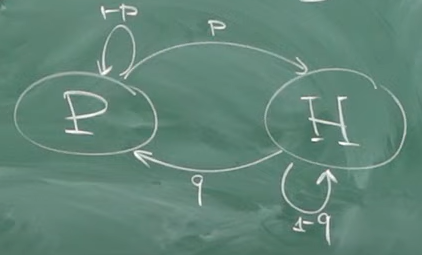
\includegraphics[width=7cm]{assets/04-descrete-random-process/probability-example-work-not-work.png}
            \end{center}


        }
    \end{enumerate}
    \begin{remark}
        $\pi_0 = P_{\xi_0}$ - начальное распределение

        $p_n (a, b) = P(\xi_n = b | \xi_{n - 1} = a)$ - вероятностости переходов. Этот набор данных однозначно определяет все распределения
    \end{remark}
\end{example}

\begin{definition}
    Цепь Маркова называется однородной, если $p_n (a, b)$ не зависят от $n$. 

    То есть вероятности переходов не зависят от времени

    \textit{Обозначение.} $p_n (a, b) = p_{ab}$
\end{definition}

\begin{remark}
    Интерпретация: есть частица, которая бегает по фазовому пространству. И мы в каждый момент фиксируем место, где находится частица.
\end{remark}

\begin{definition}
    Траектория: $\xi_0 = a_0, \xi_1 = a_1, \ldots, \xi_n = a_n$
\end{definition}

\begin{theorem}
    $P(\xi_0 = a_0, \ldots, \xi_n = a_n) = \pi_0(a_0)p_{a_0a_1}p_{a_1a_2}\ldots p_{a_{n-1}a_n}$
\end{theorem}

\begin{proof}
    Индукция по $n$

    \begin{enumerate}
        \item База индукция - определение $\pi_0$
        \item {
            Переход: $n - 1 \to n$

            $P(\xi_0 = a_0, \ldots, \xi_n = a_n) = P(\xi_n = a_n | \xi_{n - 1} = a_{n-1}, \ldots, \xi_0 = a_0) \cdot P(\xi_{n - 1} = a_{n-1}, \ldots, \xi_0 = a_0) 
            = \underbrace{P(\xi_n = a_n | \xi_{n - 1} = a_{n-1})}_{=p_{a_{n-1}a_n}} \cdot \pi_0 (a_0) p_{a_0a_1} \ldots p_{a_{n-2}a_{n-1}}$
        }
    \end{enumerate}
\end{proof}

\begin{theorem}
    Пусть $\pi_0 \, : \, Y \to [0, 1]$, т.ч. $\sum\limits_{y \in Y} \pi_0 (y) = 1$, $p \, : \, Y \times Y \to [0, 1]$, т.ч.
    $\sum\limits_{y \in Y} p_{ay} = 1 \, \forall \, a \in Y$

    Тогда существует такое пространство $(\Omega, \mathcal{F}, P)$ и последовательность $\xi_n \, : \, \Omega \to Y$, такая, что
    $\xi_n$ цепь Маркова с начальным распределением $\pi_0$ и вероятностью перехода $p_{ab}$
\end{theorem}

\textit{Обозначение. } $\pi_n = P_{\xi_n}$ и $P$ -- матрица $(p_{ab})_{a, b \in Y}$ -- это распределение системы в момент времени $n$.

\begin{theorem}
    $\pi_n = \pi_0 P^n$
\end{theorem}

\begin{proof}
    Индукция по $n$. Переход $n-1 \to n$

    $\pi_n (b) = P(\xi_n = b) = \sum\limits_{y \in Y} P(\xi_n = b | \xi_{n-1} = y) \cdot P(\xi_{n-1} = y) = \sum\limits_{y \in Y}p_{yb} \pi_{n-1}(y)$

    То есть $\pi_n = \pi_{n-1} P$
\end{proof}

\textit{Обозначение. } $p_{ab} (n) = P(\xi_{n + k} = b | \xi_k = a)$ - вероятность перехода за $n$ шагов

\begin{definition}
    $\pi \, : \, Y \to [0, 1]$ - распределение на $Y$, если $\sum\limits_{y \in Y} \pi (y) = 1$
\end{definition}

\begin{definition}
    $\pi$ - стационарное распределение для цепи Маркова, если $\pi = \pi P$
\end{definition}

\begin{example}
    Симметричное случайное блуждание на $\mathbb{Z}$, то есть $p = \frac{1}{2}$

    Пусть $\pi$ - стационарное распределение для этого блуждания

    Тогда $\frac{1}{2} \pi (n - 1) + \frac{1}{2} \pi (n + 1) = \pi (n) \Longleftrightarrow \pi (n) - \pi (n - 1) = \pi (n + 1) - \pi (n)$, то есть разность $\alpha = \pi (n) - \pi (n - 1)$ не зависит от $n$

    \begin{enumerate}
        \item $\alpha > 0$, то $\pi (n) = n\alpha + \pi (0) \rightarrow +\infty$, так не бывает
        \item $\alpha < 0$, то $\pi (n) = n\alpha + \pi (0) \rightarrow -\infty$, так тоже не бывает
        \item $\alpha = 0$ и $\pi = const$, но так тоже не бывает 
    \end{enumerate}
\end{example}

\begin{theorem}
    \textbf{Эргодическая теорема Маркова}

    $\xi_n$ - конечная цепь Маркова и $p_{ab} > 0 \, \forall \, a, b \in Y$

    Тогда существует единственное стационарное распределение и $\pi (b) = \lim_{n \to \infty} p_{ab} (n)$

    Более того, $|\pi (b) - p_{ab} (n) | \leqslant cq^n $, где $q \in (0, 1)$
\end{theorem}

\begin{proof}
    Доказательство будет с использованием теоремы Банаха о сжатии из матанализа.

    \begin{remark}
        \textit{Теормеа Банаха о сжатии}: $(X, \rho)$ -- полное метрическое пр-во, $T : X \rightarrow X$ -- сжатие с коэфф. $q \in (0, 1)$ (сжатие это $\rho(T(x), T(y)) \leq q \cdot \rho(x, y): \ \forall \ x, y \in X$).
        
        Тогда существует единственный $x^* \in X$, т.ч. $T(x^*) = x^*$ и если $x_0 \in X$ и $x_{n + 1} = T(x_n)$, то $\rho(x_n, x^*) \leq C q^n$.
    \end{remark}

    Теперь доказываем теорему:

    пусть $d$ - количество элементов в $Y$. Рассмотрим $\mathbb{R}^d$ с нормой $||x|| = |x_1| + \ldots + |x_d|$ - полное пространство

    $S = \{ x \in \mathbb{R}^d \, : \, ||x|| = 1, x_1, x_2, \ldots, x_d \geqslant 0 \}$ - замкнутое подмножество $\mathbb{R}^d$ - полное

    $T \, : \, S \to S$ и $T(x) = x^{T} P$, $\delta = \min\limits_{a, b \in Y} p_{ab} > 0$

    Проверяем, что $T$ - сжатие с $\lambda = 1 - d\delta$

    $||T_x - T_y|| \overset{z = x - y}{=} ||T_z|| = \sum\limits_{j = 1}^d |(T_z)_j| = \sum\limits_{j = 1}^d \left | \sum\limits_{k = 1}^d z_k p_{kj} \right | = 
    \sum\limits_{j = 1}^d \left | \sum\limits_{k = 1}^d z_k (p_{kj} - \delta) + \delta \underbrace{\sum\limits_{k = 1}^d z_k}_{= 0} \right | \leqslant$
    
    $\leqslant \sum\limits_{j = 1}^d \sum\limits_{k = 1}^d |z_k| (p_{kj} - \delta) = 
    \sum\limits_{k = 1}^d |z_k| \sum\limits_{j = 1}^d \underbrace{(p_{kj} - \delta)}_{=1 - \delta d = \lambda} = \lambda \sum\limits_{k = 1}^d |z_k| = \lambda ||x - y|| $
\end{proof}

\begin{remark}
    Пусть $\xi_n$ - конечная цепь Маркова, $m \in \mathbb{N}$, т.ч. $p_{ab} (m) > 0 \, \forall a, b \in Y$

    Тогда существует единственное стационарное распределение
\end{remark}

\begin{definition}
    Состояние $b$ достижимо из $a$, если $\exists \, n \in \mathbb{N}$, т.ч. $p_{ab} (n) > 0$
\end{definition}

\begin{definition}
    Состояния $a$ и $b$ сообщающиеся, если $a$ достижимо из $b$, а $b$ достижимо из $a$
\end{definition}

\begin{definition}
    Состояние $a$ существенное, если $\forall \, b$, достижимого из $a$ - состояния $a$ и $b$ сообщающиеся
\end{definition}

\textit{Обозначение. } $f_{a} (n) = P(\xi_n = a | x_{n - 1} \neq a, \xi_{n - 2} \neq a, \ldots, \xi_1 \neq a, \xi_0 = a)$ - вероятность, стартовав из $a$, впервые вернуться назад на $n$-ном шаге.

$F_a = \sum\limits_{n = 1}^\infty f_{a} (n)$ - вероятность возврата назад в $a$

\begin{definition}
    $a$ - возвратное состояние, если $F_a = 1$
\end{definition}

\begin{definition}
    $a$ - нулевое состояние, если $p_{aa} (n) \rightarrow 0$
\end{definition}

\begin{theorem}
    \textbf{Критерий возвратности}

    $a$ - возвратное $\Longleftrightarrow$ $(*) = P_a = \sum\limits_{n = 1}^\infty p_{aa} (n)$ расходится

    И если $a$ не возвратное, то $F_a = \frac{P_a}{1 + P_a}$
\end{theorem}

\begin{lemma}
    $c_n \geqslant 0$ и $\sum_{n=0}^{\infty} c_n = +\infty$. 

    Тогда $\lim\limits_{x\to 1-} \sum_{n=0}^{\infty} c_nx^n = +\infty$
\end{lemma}

\begin{proof} Леммы.


    Берём $n$, т.ч. $\sum_{k=0}^{n} c_k > A$, а $\sum_{k=1}^{n} \rightarrow_{x\to 1-} \sum_{n=0}^{n}c_k$. Тогда
    $\underbrace{\sum_{k=0}^{n} c_kx^k}_{\leqslant \sum_{n=0}^{\infty} c_nx^n} > A - 1$ при $x$ близких к 1
\end{proof}

\begin{proof}
    Теоремы.

    Давайте считать, что $p_{aa} (0) = 1$ и $f_a (0) = 0$

    $\mathcal{F} (z) = \sum_{n=0}^{\infty} f_a (n) z^n$, сходится при $|z| \leqslant 1$

    $\mathcal{P} (z) = \sum_{n=0}^{\infty} p_{aa} (n)z^n$, сходится при $|z| < 1$

    $p_{aa} (n) = \sum_{k = 0}^{n} f_a (k) p_{aa} (n - k)$ - верно при $n \geqslant 1$

    Тогда $\mathcal{P} (z) = \mathcal{F} (z) \mathcal{P} (z)$ - почти верное равенство, надо ещё подкорректировать при $z^0$.
    Получим $\mathcal{P} (z) = \mathcal{F} (z) \mathcal{P} (z) + 1 \implies \mathcal{F} (z) = \frac{\mathcal{P} (z) - 1}{\mathcal{P} (z)}$. Давайте устремим $z \to 1$
    
    $\underbrace{\lim\limits_{z \to 1-} \mathcal{F} (z)}_{=F_a} = \lim\limits_{z \to 1-} \frac{\mathcal{P} (z) - 1}{\mathcal{P} (z)} \overset{\text{если $(*)$ сходится}}{=} \frac{P_a}{P_a + 1}$.

    А если расходится, то смотрим на $\underbrace{(1 - \mathcal{F} (z))}_{\to 1 - F_a} \underbrace{\mathcal{P} (z)}_{\to 1 + P_a} = 1$. Отсюда получаем, что $F_a = 1$
\end{proof}

\begin{consequence}
    Если $a$ не возвратное $\implies$ $a$ - нулевое
\end{consequence}

\begin{theorem}
    \textbf{Теорема солидарности}

    $a$ и $b$ сообщающиеся состояния

    Тогда они возвратны/не возвратны (нулевые/не нулевые) одновременно
\end{theorem}

\begin{proof}
    $a$ и $b$ сообщающиеся, значит $\exists \,  j, k \in \mathbb{N} \, : \, p_{ab} (j) > 0$ и $p_{ba} (k) > 0$

    $p_{aa} (n + j + k) \geqslant p_{ab} (j) p_{bb} (n) p_{ba} (k)$ и $\sum\limits_{n = 1}^\infty p_{aa} (n + j + k) \geqslant p_{ab} (j) p_{ba} (k) \sum\limits_{n = 1}^\infty p_{bb} (n)$

    Отсюда всё следует, потому что:

    Если $p_{aa} (n + j + k) \rightarrow 0$, то $p_{bb} (n) \rightarrow 0$
    
\end{proof}

\begin{theorem}
    \textbf{ЗБЧ для цепей Маркова}

    $\varepsilon > 0$ и цепь удовлетворяет условию теоремы Маркова, $\pi$ - стационарное распределение  
    
    Тогда 
    \begin{enumerate}
        \item $P\left( \left| \frac{\nu_a (n)}{n} - \pi (a) \right| \geqslant \varepsilon \right) \rightarrow 0$
        \item $P\left( \left| \frac{\nu_{ab} (n)}{n} - \pi (a) p_{ab} \right| \geqslant \varepsilon \right) \rightarrow 0$
    \end{enumerate}

    Здесь $\nu_a (n)$ - количество значений $\xi_1, \ldots, \xi_n$, равных $a$
    
    $\nu_{ab} (n)$ - количество пар $ab$ на соседних позициях
\end{theorem}

\begin{proof}
    Пусть $\eta_k = 
    \begin{cases}
        1, & \text{если $\xi_k = a$}\\
        0, & \text{иначе}    
    \end{cases}$

    $\tilde{\eta_k} = 
    \begin{cases}
        1, & \text{если $\xi_k = a$ и $\xi_{k + 1} = b$}\\
        0, & \text{иначе}    
    \end{cases}$

    Тогда $\nu_a (n) = \eta_1 + \ldots + \eta_n$ и $\nu_{ab} (n) = \tilde{\eta_1} + \ldots + \tilde{\eta_n}$

    Посмотрим на $\mathbb{E} \eta_k = P(\xi_k = a) = \sum\limits_{y \in Y} \pi_0(y) \underbrace{p_{ya} (k)}_{\rightarrow \pi (a)} \rightarrow \pi (a)$

    Значит $\mathbb{E} \frac{\nu_a (n)}{n} = \frac{1}{n} \sum\limits_{n=1}^{n} \mathbb{E} \eta_k \rightarrow \pi (a)$

    По аналогии считаем для второй ситуации:

    $\mathbb{E} \tilde{\eta_k} = P(\xi_k = a, \xi_{k + 1} = b) = \sum\limits_{y \in Y} \pi_0 (y) \underbrace{p_{ya}}_{\rightarrow \pi (a)} (k) p_{ab}  \rightarrow \pi (a) p_{ab}$

    $\mathbb{E} \frac{\eta_{ab} (n)}{n} = \frac{1}{n} \sum\limits_{k=1}^{n} \mathbb{E} \tilde{\eta_k}$

    Пишем Чебышёва: $P \left( \left| \frac{\nu_a (n)}{n} - \mathbb{E} \frac{\nu_a (n)}{n} \right| \geqslant \varepsilon \right) \leqslant \frac{\mathbb{D} \left( \frac{\nu_a (n)}{n} \right)}{\varepsilon^2} = \frac{\mathbb{D} \nu_a (n)}{\varepsilon^2 n^2}$

    $\mathbb{D} \nu_a (n) = \mathbb{D} (\sum_{k=1}^{n} \eta_k) = \underbrace{\sum_{k = 1}^{n} \mathbb{D} \eta_k}_{\leqslant n} + 2\sum\limits_{i < j} cov (\eta_i, \eta_j)$

    Давайте как-то оценим ковариацию:

    $cov (\xi_i, \xi_j) = \mathbb{E} (\eta_i, \eta_j) - \mathbb{E} \eta_i \mathbb{E} \eta_j$

    Здесь $\mathbb{E} (\eta_i \eta_j) = P(\xi_i = a, \xi_j = a) = \sum\limits_{y \in Y} \pi_0 (y) \underbrace{p_{ya} (i)}_{= \pi (a) + \mathcal{O}(\lambda^i)} \underbrace{p_{aa} (j - i)}_{\pi (a) + \mathcal{O} (\lambda^{j - i})} = \pi^2 (a) + \mathcal{O} (\lambda^i) + \mathcal{O} (\lambda^{j - i}) + \mathcal{O} (\lambda^i)$

    $\mathbb{E} \eta_i = P(\xi_i = a) = \sum\limits_{y \in Y} \pi_0 (y) \underbrace{p_{ya} (i)}_{\pi (a) + \mathcal{O} (\lambda^i)} = \pi (a) + \mathcal{O} (\lambda^i)$ 

    Мы поняли, что $cov (\eta_i, \eta_j) = \mathcal{O} (\lambda^i) + \mathcal{O} (\lambda^{j - i})$ и эти ковариации надо просуммировать

    $\sum\limits_{i < j} cov (\eta_i, \eta_j) = \sum\limits_{i < j} \left(\mathcal{O} (\lambda^i) + \mathcal{O} (\lambda^{j - i})\right) = \mathcal{O} (n)$

    Осталось заметить, что $\{ \left| \frac{\nu_a (n)}{n} - \pi (a) \right| \geqslant \varepsilon \} \subset \{ \left| \frac{\nu_a (n)}{n} - \mathbb{E} \frac{\nu_a (n)}{n} \right| \geqslant \frac{\varepsilon}{2} \}$.

    Мы поностью доказали первый пункт, во втором аналогично оценивается дисперсия
\end{proof}

\Subsection{Случайные блуждания}

\begin{theorem}
    Рассмотрим блуждание по целочисленной прямой

    Блуждание возвратно $\Longleftrightarrow p = \frac{1}{2}$
\end{theorem}

\begin{proof}
    Возвратность $\Longleftrightarrow$ $\sum\limits_{n=1}^\infty p_{00} (n) = +\infty$

    $p_{00} (2n - 1) = 0$

    $p_{00} (2n) = p^n (1-p)^n \binom{2n}{n} \sim \frac{4^n}{\sqrt{\pi n}} (p(1-p))^n $

    Если $p \neq \frac{1}{2}$, то $4p (1 - 1p) < 1$ и $p_{00} (2n) \leqslant C (4p(1-p))^n $ - сходящаяся геометрическая прогрессия $implies$ невозвратность.

    Если $p = \frac{1}{2}$, то $p_{00} (n) \sim \frac{1}{\sqrt{\pi n}} \implies$ ряд расходится $\implies$ возвратность.
\end{proof}

\begin{remark}
    
Симметричное блуждание по $\mathbb{Z}$. Возьмём $\eta_k$ независимые одинаково распределённые случайные величины, т.ч. $P(\eta_k = a) = P(\eta_k = -a)$ и $\xi_n = \eta_1 + \ldots + \eta_n$

\end{remark}

\begin{theorem} Условия берутся из замечания выше.


    Если $\eta_1$ имеет матожидание, то блуждание возвратно.
\end{theorem}

\begin{proof}
    $G$ - производящая функция для $\eta_1$. То есть $G(z) = \sum\limits_{k \in \mathbb{Z}} P(\eta_1 = k) z^k$

    $G_{\xi_n} (z) = (G(z))^n$. Нас интересует $p_{00} (n) = P(\xi_n = 0)$ - коэффициент при $z^0$ в $G_{\xi_n}$ - подставить 0 в ряд Лорана не можем. Зато умеем считать вычет:

    $p_{00} (n) = \frac{1}{2\pi i} \int\limits_{|z| = 1} \frac{G^n (z)}{z} \, dz$

    $\sum\limits_{n=0}^\infty p_{00} (n)x^n = \sum\limits_{n = 0}^\infty \frac{1}{2\pi i} \int\limits_{|z| = 1} \frac{G^n (z) x^n}{z} \, dz \overset{?}{=} \frac{1}{2\pi i} \int\limits_{|z| = 1} \frac{1}{z} \underbrace{\sum\limits_{n = 0}^\infty x^n G^n (z)}_{= \frac{1}{1 - xG(z)}} \, dz =_{z = e^{it}} $
    
    $= \frac{1}{2\pi} \int_{-\pi}^\pi \frac{dt}{1 - xG(e^{it})} dt = \frac{1}{\pi} \int_0^\pi \frac{dt}{1 - xG(e^{it})}dt \overset{{*}}{=} \frac{1}{\pi} \int_0^\pi \frac{dt}{1 - x + o(xt)}dt \geqslant \frac{1}{\pi} \int_0^\pi \frac{dt}{1 - x + xt}dt =$
    
    $= \frac{1}{\pi} \frac{\ln (1 - x + xt)}{x} \bigg |_{t=0}^{t = \pi} \rightarrow_{x \to 1-} +\infty$ $\implies$ ряд расходится, тогда блуждание возвратно.

    $(?): $ по теореме Фубини, если ряд из подинтегрального выражения сходится, то можно переставлять.

    $(*) \, : \, G(1 + s) = G(1) + \underbrace{G' (1)}_{\mathbb{E} \eta_1} \cdot s + o(s) = 1 + o(s)$. Тогда $G(e^{it}) = 1 + o(e^{it} - 1) = 1 + o(t)$
\end{proof}

\begin{remark}
    На самом деле все состояния нулевые.

    $\underbrace{p_{00} (n)}_{? \, : \, \rightarrow 0} = \frac{1}{2\pi i} \int\limits_{|z| = 1} \frac{G^n (z)}{z} \, dz \rightarrow \frac{1}{2\pi i} \int\limits_{|z| = 1} \frac{\lim_{n\to \infty} G^n (z)}{z} \, dz$

    $\left| G(z) \right| = \left| \sum\limits_{n \in \mathbb{Z}} P(\eta = n) z^n \right| \leqslant \sum\limits_{n \in \mathbb{Z}} P(\eta = n) |z|^n = \sum\limits_{n \in \mathbb{Z}} P(\eta = n) = 1$

    Надо показать, что при почти всех $t$: $|G(e^{it})| < 1$:

    При $|G(e^{it})| < 1$, то $\lim_{n \to \infty} G^n(z) = 0$

    При $|G(e^{it})| \leq 1$, то надо показать, что такое случается для счетного кол-ва $t$-шек. 

    $\left| \sum P(\eta = n) e^{int} \right| = \sum P(\eta = n)$

    Если $P(\eta = n) > 0$ и $P(\eta = k) > 0$, то $\arg e^{int} = \arg e^{ikt}$. То есть $nt = kt + 2\pi m \implies t = 2\pi \frac{m}{n - k} \in \pi \mathbb{Q}$ - счётное множество. Значит множество точек, в которых знак нестрогий - счётно.

    Значит $G^n (z) \rightarrow 0$ почти везде
\end{remark}

\begin{theorem}
    \textbf{Теорема Пойя о возвращении}

    Рассматриваем решётку $\mathbb{Z}^d$, вероятность перейти в соседние узлы $\frac{1}{2d}$, то есть аналог случайного блуждания на прямой

    Такое блуждание возвратно $\Longleftrightarrow$ $d \leqslant 2$
\end{theorem}

\begin{proof}
    \begin{enumerate}
        \item $d = 1$ обсуждали
        \item {
            $d = 2$. По критерию возвратности, нам достаточно доказать, что $\sum\limits_{n=1}^\infty p_{00} (n) = +\infty$

            $p_{00} (n) = 0$, если $n$ нечётное. 
            
            Повёрнем оси на $45^{\circ}$. Исходные оси $(x, y)$, а повёрнутые $(x', y')$


            \begin{center}
                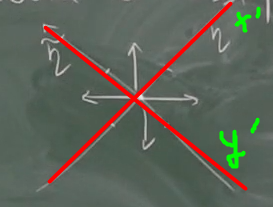
\includegraphics[width=7cm]{assets/04-descrete-random-process/poya-theorem-coordinates.png}
            \end{center}

            То есть $P(x' = x' + 1, y' = y' + 1) = P(x = x + 1) = \frac{1}{4} = P(x' = x' + 1) \cdot P(y' = y' + 1)$

            $P(x' = x' + 1) = P(x = x + 1) + P(y = y - 1) = \frac{1}{2}$

            $P(y' = y + 1) = \frac{1}{2}$

            То есть блуждание проекций на оси $x'$ и $y'$ независимы. Значит $p_{00}(n) =
            \left( \binom{2n}{n} \cdot \frac{1}{2^{2n}} \right)^2 \sim \left( \frac{1}{\sqrt{\pi n}} \right)^2 = \frac{1}{\pi n}$ - а такой ряд расходится
        }
        \item {
            $d = 3$

            Если $n$ нечётно, то всё ещё $p_{00} (n) = 0$

            По каждой координате мы делаем одинаковое число шагов в обоих направлениях: 
            
            $p_{00} (2n) = \sum\limits_{i + j \leqslant n} \binom{2n}{i, i, j, j, n - i -j, n - i - j} \cdot \frac{1}{6^{2n}} = \sum\limits_{i + j \leqslant n} \frac{(2n)!}{(i!j!(n-i-j)!)^2} \cdot \frac{1}{6^{2n}} = 
            \binom{2n}{n} \sum\limits_{i + j \leqslant n} \left( \frac{n!}{i!j!(n - i - j)!} \right)^2 \cdot \frac{1}{6^{2n}} \overset{*}{\leqslant} \underbrace{\frac{\binom{2n}{n}}{6^{2n}} \cdot 3^n}_{\sim \frac{1}{\sqrt{\pi n} \cdot \frac{1}{3^n}}} \cdot \max \binom{n}{i, j, n - i - j}$

            При этом $\sum\limits_{i + j \leqslant n} \left( \frac{n!}{i!j!(n - i - j)!} \right) = (1 + 1 + 1)^n = 3^n \implies \sum\limits_{i + j \leqslant n} \left( \frac{n!}{i!j!(n - i - j)!} \right)^2 \leqslant \max \binom{n}{i, j, n - i - j} \cdot \sum\limits_{i + j \leqslant n} \left( \frac{n!}{i!j!(n - i - j)!} \right) \sim (*)$

            Осталось разобраться с максимумом: $\max \sim 3^n \cdot \frac{3\sqrt{3}}{2 \pi n}$ -- достигается, когда $i, \ j, \ (n - i - j)$ равны, либо отличаются на 1 (если $n$ не делится на 3), и остается записать формулу Стирлинга.

            $(*) \sim \frac{3\sqrt{3}}{2 (\pi n)^{\frac{3}{2}}} \implies $ ряд сходится, то есть нет возвратности.
        }
        \item {
            Что делать с размерностью $\geqslant 4$.
            
            Выберем первые 3 координаты и будем следить что происодит с проекцией на эти координаты. 
            Если мы двигаемся по ним - происходит смещение. Если по другим, то мы стоим на месте. Эти остановки не бывают бесконечно долгими, то есть получили блуждание по 6 направлениям.

            То есть проекция возвращается назад с вероятностью $< 1$, а значит и глобальное тоже не возвратное
        }
    \end{enumerate}
\end{proof}

\begin{remark}
    \textbf{Случайное блуждание с отталкивающим экраном}

    Есть блуждание по прямой и где-то стоит отталкивающий экран. То есть если мы врезались в стенку, то отскочили от неё с вероятностью 1
\end{remark}

\begin{remark}
    \textbf{Случайное блуждание с поглащающим экраном}
    
    Есть блуждание по прямой, где-то стоит экран, попав в него, мы попадаем в петлю, из которой не выбираемся
\end{remark}

\begin{example}
    \textbf{Задача о разорении}

    $A$ монет у первого, $B$ монет в второго

    Это случайное блуждание с поглащающими экранами. Блуждание по прямой, поглащающие экраны в точках $-A$ и $B$.
    Между ними мы смещаемся с вероятностями $p$ и $q = 1 - p$

    $\beta_k (x)$ - вероятность оказаться в $B$ через $k$ шагов, если сейчас наша фишка находится в $x$

    Переходы: $x \overset{p}{\rightarrow} x + 1$, $x \overset{q}{\leftarrow} x - 1$

    То есть $\beta_k (x) = p \beta_{k - 1} (x + 1) + q \beta_{k - 1} (x - 1)$

    А ещё $\beta_k (x) \leqslant \beta_{k + 1} (x) \leqslant 1$

    Пусть $\beta (x) = \lim\limits_{k \to \infty} \beta_k (x)$

    Тогда $\beta (x) = p \beta (x + 1) + q \beta (x - 1)$ - рекуррента. А ещё $\beta (B) = 1$ и $\beta (-A) = 0$

    Общее решение $pt^2 - t + q = 0$, здесь корни $1$ и $\frac{q}{p}$

    Тогда $\beta (x) = a + b \cdot \left( \frac{q}{p} \right)^x$
    
    $\beta (-A) = a + b \left( \frac{q}{p} \right)^{-A} \implies a = -b \left( \frac{q}{p}\right)^{-A}$

    $\beta (B) = a + b \left( \frac{q}{p} \right)^B = b \left( \frac{q}{p} \right)^B - b \left( \frac{q}{p} \right)^{-A}$, откуда $a$ и $b$ выражаются
\end{example}

\Subsection{Процесс восстановления}

\begin{definition}
    $\xi_1, \xi_2, \ldots$ - неотрицательные, одинаково распределённые независимые случайные величины

    $S_0 = 0, S_n = \xi_1 + \xi_2 + \ldots + \xi_n$

    $\xi_i$ - время работы прибора $i$, после его поломки, его мнгновенно меняют на следующий

    $\Phi (t) = P(S_n \leqslant t)$ - функция распределения для $S_n$

    $\nu (t)$ - количество приборов, использованных на момент времени $t$. То есть $\nu (t) = n$, если $S_{n-1} \leqslant t < S_n$

    $P(\nu (t) = n) = P(S_{n - 1} \leqslant t < S_n) = \Phi_{n-1} (t) - \Phi_n (t)$

    Функция восстановления $\mathcal{N} (t) = \mathbb{E} \nu (t)$
\end{definition}

\begin{theorem}
    $\mathcal{N} (t) = \sum\limits_{n = 1}^{\infty} \Phi_n (t)$, если ряд в правой части сходится
\end{theorem}

\begin{proof}
    $\mathcal{N} (t) = \mathbb{E} \nu (t) = \sum\limits_{n = 1}^\infty n P(\nu (t) = n) = \sum\limits_{n = 1}^\infty n (\Phi_{n - 1} (t) - \Phi_n (t))$ - нужно понять, что это правая часть в утвеждении теоремы

    Смотрим на частичную сумму: $\sum\limits_{n = 1}^m n (\Phi_{n - 1} - \Phi_n) = (\Phi_0 - \Phi_1) + 2 (\Phi_1 - \Phi_2) + \ldots + m (\Phi_{m - 1} - \Phi_m) = \Phi_0 + \Phi_1 + \ldots + \Phi_{m-1} + \underbrace{m\Phi_m}_{\overset{?}{\rightarrow} 0}$

    Если ряд $\sum\limits_{n = 1}^\infty \Phi_n (t)$ сходится, тогда $\underbrace{\Phi_n + \Phi_{n+1} + \ldots + \Phi_{2n}}_{\geqslant n \Phi_{2n}} \rightarrow 0$, а ещё $\Phi_{n + 1} \leqslant \Phi_n$. А значит $\Phi_n = o \left( \frac{1}{n} \right)$
\end{proof}

\textbf{Дальше все $\xi_n$ будут целозначные}

\begin{remark}
    $\Phi_n (t) = \sum\limits_{k \leqslant t} P(S_n = k)$

    $\mathcal{N} (t) = \sum\limits_{n=1}^\infty \Phi_n (t) = \sum\limits_{n = 1}^\infty \sum\limits_{k \leqslant t} P(S_n = k) = \sum\limits_{k \leqslant t} \underbrace{\sum\limits_{n = 1}^\infty P(S_n = k)}_{=q_k}$
\end{remark}

\begin{example}
    Прибор либо работает единицу времени с вероятностью $p$, либо мнгновенно ломается с вероятностью $q = 1 - p$. Считаем, что $0 < p \leqslant 1$

    $P(S_n = k) = \underbrace{\binom{n}{k}}_{\leqslant n^k} p^k q^{n - k} \leqslant q^n \left( \frac{np}{q} \right)^k$

    Тогда $q_k = \sum\limits_{n = 1}^\infty P(S_n = k) \leqslant \sum\limits_{n=1}^\infty q^n \left( \frac{np}{q} \right)^k = \frac{q}{1 - q} \left( \frac{np}{q} \right)^k = n^k \left(\frac{p}{q}\right)^{k - 1} < +\infty$
\end{example}

\begin{theorem}
    Если $P(\xi_1 = 0) < 1$, то $\mathcal{N} (t)$ конечно
\end{theorem}

\begin{proof}
    $\{ \xi_1 = 0 \} = \bigcap\limits_{m=1}^\infty \{ \xi_1 \leqslant \frac{1}{m} \} \implies P(\xi_1 = 0) = \lim\limits_{m \to \infty} P(\xi_1 \leqslant \frac{1}{m}) \implies \exists \, m \, : \, q = P(\xi_1 \leqslant \frac{1}{m}) < 1$ - потому что предел $< 1$

    $\tilde{\xi_k} = 
    \begin{cases}
        0, & \text{если $\xi_k \leqslant \frac{1}{m}$ - это с вероятностью $q$} \\
        1, & \text{если $\xi_k > \frac{1}{m}$}    
    \end{cases}$

    Поэтому из примера $\tilde{\mathcal{N}} (t)$ конечно

    $\tilde{\xi_k} \leqslant m \xi_k \implies \tilde{S_n} \leqslant mS_n \implies P(\tilde{S_n} \leqslant t) \geqslant P(S_n \leqslant \frac{t}{m}) \implies \tilde{\Phi_n} (t) \geqslant \Phi_n \left(\frac{t}{m}\right) $

    Значит $\mathcal{N} \left( \frac{t}{m} \right) = \sum\limits_{n=1}^\infty \Phi_n \left( \frac{t}{m} \right) \leqslant \sum\limits_{n=1}^\infty \tilde{\Phi_n} (t) = \tilde{\mathcal{N}} (t) < +\infty \implies \mathcal{N} (t)$ конечна при всех $t$
\end{proof}

\begin{definition}
    $\xi$ имеет решётчатое распределение с шагом $h \geqslant 0$, если $\xi (\Omega) \subset a + h\mathbb{Z}$ для некоторого $a \in \mathbb{R}$, а для больших $h$ это неверно

    \begin{remark}
        Рассмотрим целочисленную случайную величину с шагом решётки 1.

        Тогда $ \left| G_{\xi} (z) \right| < 1$, если $|z| \leqslant 1$ и $z \neq 1$

        $\left| G_{\xi} (z) \right| = \left| \sum\limits_{n=0}^\infty P(\xi = n) z^n \right| \leqslant \sum\limits_{n=0}^\infty P(\xi = n) |z^n| \leqslant \sum\limits_{n=0}^\infty P(\xi = n) = 1$

        Правое неравенство обращается в равенство, если $|z| = 1$

        Левое неравенство обращается в равенство, если модуль суммы равен сумме модулей, то есть все $z$ имеют один и тот же аргумент $\implies z = e^{it}$ и $z^n = z^{int}$. Тогда 
        $nt - mt = 2\pi k \implies n - m = \frac{2\pi}{t} \cdot k < \frac{2\pi}{t} \mathbb{Z}$, а так как $0 < t < 2\pi$, то мы получили решётку с $h > 1$
    \end{remark}
\end{definition}

\begin{theorem}
    \textbf{Теорема восстановления}

    $\mathcal{N} (t + s) - \mathcal{N} (t) \rightarrow_{t \to \infty} \frac{S}{\mathbb{E} \xi_1}$

    Если:
    \begin{enumerate}
        \item $\xi$ имеет нерешетчатое распределение
        \item $\xi$ имеет решетчатое распределение с шагом $h$ и $S = kh$, где $k \in \mathbb{N}$ 
    \end{enumerate}
\end{theorem}

\begin{proof}
    Доказываем лишь для целозначных случайных величин $\xi_k$, тогда можем считать, то $h = 1$

    Тогда достаточно доказать, что $\underbrace{\mathcal{N} (t + 1)}_{=\sum\limits_{k \leqslant t + 1} q_k} - \underbrace{\mathcal{N} (t)}_{=\sum\limits_{k \leqslant t} q_k} \rightarrow \frac{1}{\mathbb{E} \xi_1}$

    То есть нам надо доказать, что $q_k \rightarrow_{k \to \infty} \frac{1}{\mathbb{E} \xi_1}$

    $Q(z) = \sum\limits_{k = 0}^\infty q_k z^k$. Поймём, что $Q(z) = \frac{1}{1 - G(z)}$, где $G(z)$ - производящая функция для $\xi_1$

    $Q(z) = \sum\limits_{k = 0}^\infty q_k z^k = \sum\limits_{k=0}^\infty \sum\limits_{n = 0}^\infty P(S_n = k) z^k = \sum\limits_{n=0}^\infty \underbrace{\sum\limits_{k = 0}^\infty P(S_n = k) z^k}_{\text{производящая функция для $S_n$}}
    = \sum\limits_{n = 0}^\infty G^n (z) = \frac{1}{1 - G(z)}$ - верно при $|z| \leqslant 1$ и $z \neq 1$

    \begin{lemma}
        $q_n - q_{n-1} \rightarrow 0$
    \end{lemma}
    
    \begin{proof}
        Производящая функция для $q_n - q_{n-1} = (1-z) Q (z) = \frac{1-z}{1 - G(z)}$

        Значит $q_n - q_{n-1} = \frac{1}{2\pi i} \int\limits_{|z| = r} \underbrace{\frac{1 - z}{1 - G(z)}}_{\text{непрерывна в $|z| \leqslant 1$}} \frac{dz}{z^{n+1}} = \frac{1}{2\pi i} \int\limits_{|z| = 1} \frac{1 - z}{1 - G(z)} \frac{dz}{z^{n + 1}} =
        \frac{1}{2\pi} \int\limits_0^{2\pi} \underbrace{\frac{1 - e^{it}}{1 - G(e^{it})}}_{\text{непрерывна, ограничена}} e^{-int} \, dt \\
        \overset{\text{лемма Римана-Лебега}}{\rightarrow} 0$
    \end{proof}

    \begin{lemma}
        $\sum\limits_{k = 0}^n q_{n - k}r_k = 1$, где $r_k = \sum\limits_{j = k + 1}^\infty P(\xi_1 = j)$
    \end{lemma}

    \begin{proof}
        $Q(z) \frac{1 - G(z)}{1 - z} = \frac{1}{1 - z}$

        Посмотрим на коэффициенты при $z^n$ в левой части равенства - это свёртка. То есть достаточно понять, что $r_k$ появляются из $\frac{1 - G(z)}{1 - z}$

        $\frac{1 - G(z)}{1 - z} = \frac{G(1) - G(z)}{1 - z} = \sum\limits_{n = 0}^\infty \frac{P(\xi_1 = n) (1 - z^n)}{1 - z} = \sum\limits_{n = 1}^\infty P(\xi_1 = n) \cdot (1 + z + z^2 + \ldots + z^{n - 1}) = \sum\limits_{k = 0}^\infty r_k z^k$
    \end{proof}

    \begin{consequence}
        $q_n \leqslant \frac{1}{r_0}$
    \end{consequence}

    Выберем сходящуюся подпоследовательность $q_{k_m} \rightarrow_{m \to \infty} s \implies q_{k_{m} \pm l} \rightarrow_{m \to \infty} s$

    Мы знаем, что $1 = \sum\limits_{k = 0}^n q_{n - k}r_k \geqslant \sum\limits_{k = 0}^N q_{n - k}r_k \rightarrow s \sum\limits_{k = 0}^N r_k \implies 1 \geqslant s \sum\limits_{k = 0}^N r_k \rightarrow s \mathbb{E} \xi_1 \implies \frac{1}{\mathbb{E} \xi_1} \geqslant s$

    \begin{enumerate}
        \item {
            Если $\mathbb{E} \xi_1 = +\infty$, то $\sum\limits_{k = 1}^\infty r_k = \mathbb{E} \xi_1 = +\infty \implies \sum\limits_{k = 0}^N r_k$ сколь угодно большая, тогда $s = 0$

            Можно считать, что $s = \overline{\lim} q_k$, а ещё $q_k \geqslant 0 \implies \underline{\lim} q_k \geqslant 0 \implies \lim = 0$
        }
        \item {
            Если $\mathbb{E} \xi_1 < +\infty$, тогда $\sum\limits_{k = 1}^\infty r_k = \mathbb{E} \xi_1 < +\infty \implies r_k \rightarrow 0 \implies r_k$ ограничены, $r_k \leqslant M$

            $1 = \sum\limits_{k = 0}^n q_{n - k} r_k = \sum\limits_{k = 0}^N q_{n - k} r_k + \underbrace{\sum\limits_{k = N + 1}^n q_{n - k}r_k}_{M \sum\limits_{k = N + 1}^n r_k < \varepsilon M} < \varepsilon M + \sum\limits_{k = 0}^N q_{n - k}r_k 
            \rightarrow_{n = k_m} \varepsilon M + s\sum\limits_{k = 0}^N r_k \leqslant \varepsilon M + s\mathbb{E} \xi_1 \implies 1 \leqslant s \mathbb{E} \xi_1 \implies \underline{\lim} \geqslant \frac{1}{\mathbb{E} \xi_1}$ 

            А ещё $\sum\limits_{k = 0}^N q_{n - k}r_k \rightarrow s \sum\limits_{k = 0}^N r_k \implies 1 \geqslant s \sum\limits_{k = 0}^N r_k \rightarrow s \mathbb{E} \xi_1 \implies \frac{1}{\mathbb{E} \xi_1} \geqslant s$ - получили неравенство и на верхрний предел
        }
    \end{enumerate}
\end{proof}

\begin{consequence}
    $\frac{\mathcal{N} (t)}{t} \rightarrow \frac{1}{\mathbb{E} \xi_1}$
\end{consequence}

\begin{proof}
    Теорема Штольца
\end{proof}

\begin{remark}
    Парадокс времени восстановления

    $P(\xi_{\nu (t)} > x) \geqslant P(\xi_1 > x)$
\end{remark}